%%%
%
% $Autor: Siddhanth Sharma $
% $Date: 2026-04-27 12:00:00Z $
% $File: ETS.tex $
% $Version: 1 $
%
% Project: Time Series CPI Forecasting
%
%%%

\chapter{Error, Trend, and Seasonality (ETS)}
\label{ch:ets}

\section{Description}
The Error, Trend, and Seasonality (ETS) framework represents a highly generalized, robust class of exponential smoothing methods used extensively for point forecasting and statistical analysis of time series data. In contrast to ARIMA models—which rely on describing linear autocorrelations between past and future observations—the ETS framework adopts an intuitive state-space formulation. It decomposes the time series sequence into an underlying ``level,'' overlaid by a ``trend'' component and a ``seasonal'' component. Figure~\ref{fig:ets_decomposition} visually demonstrates this fundamental decomposition of the actual CPI dataset. It applies exponentially decreasing weights to past observations, implying that recent history holds more predictive power than distant history. By characterizing the Error (E), Trend (T), and Seasonality (S) as mathematically discrete states that evolve over time, it establishes a probabilistic foundation capable of generating robust forecast intervals for almost any underlying data-generating process.

\begin{figure}[htbp]
    \centering
    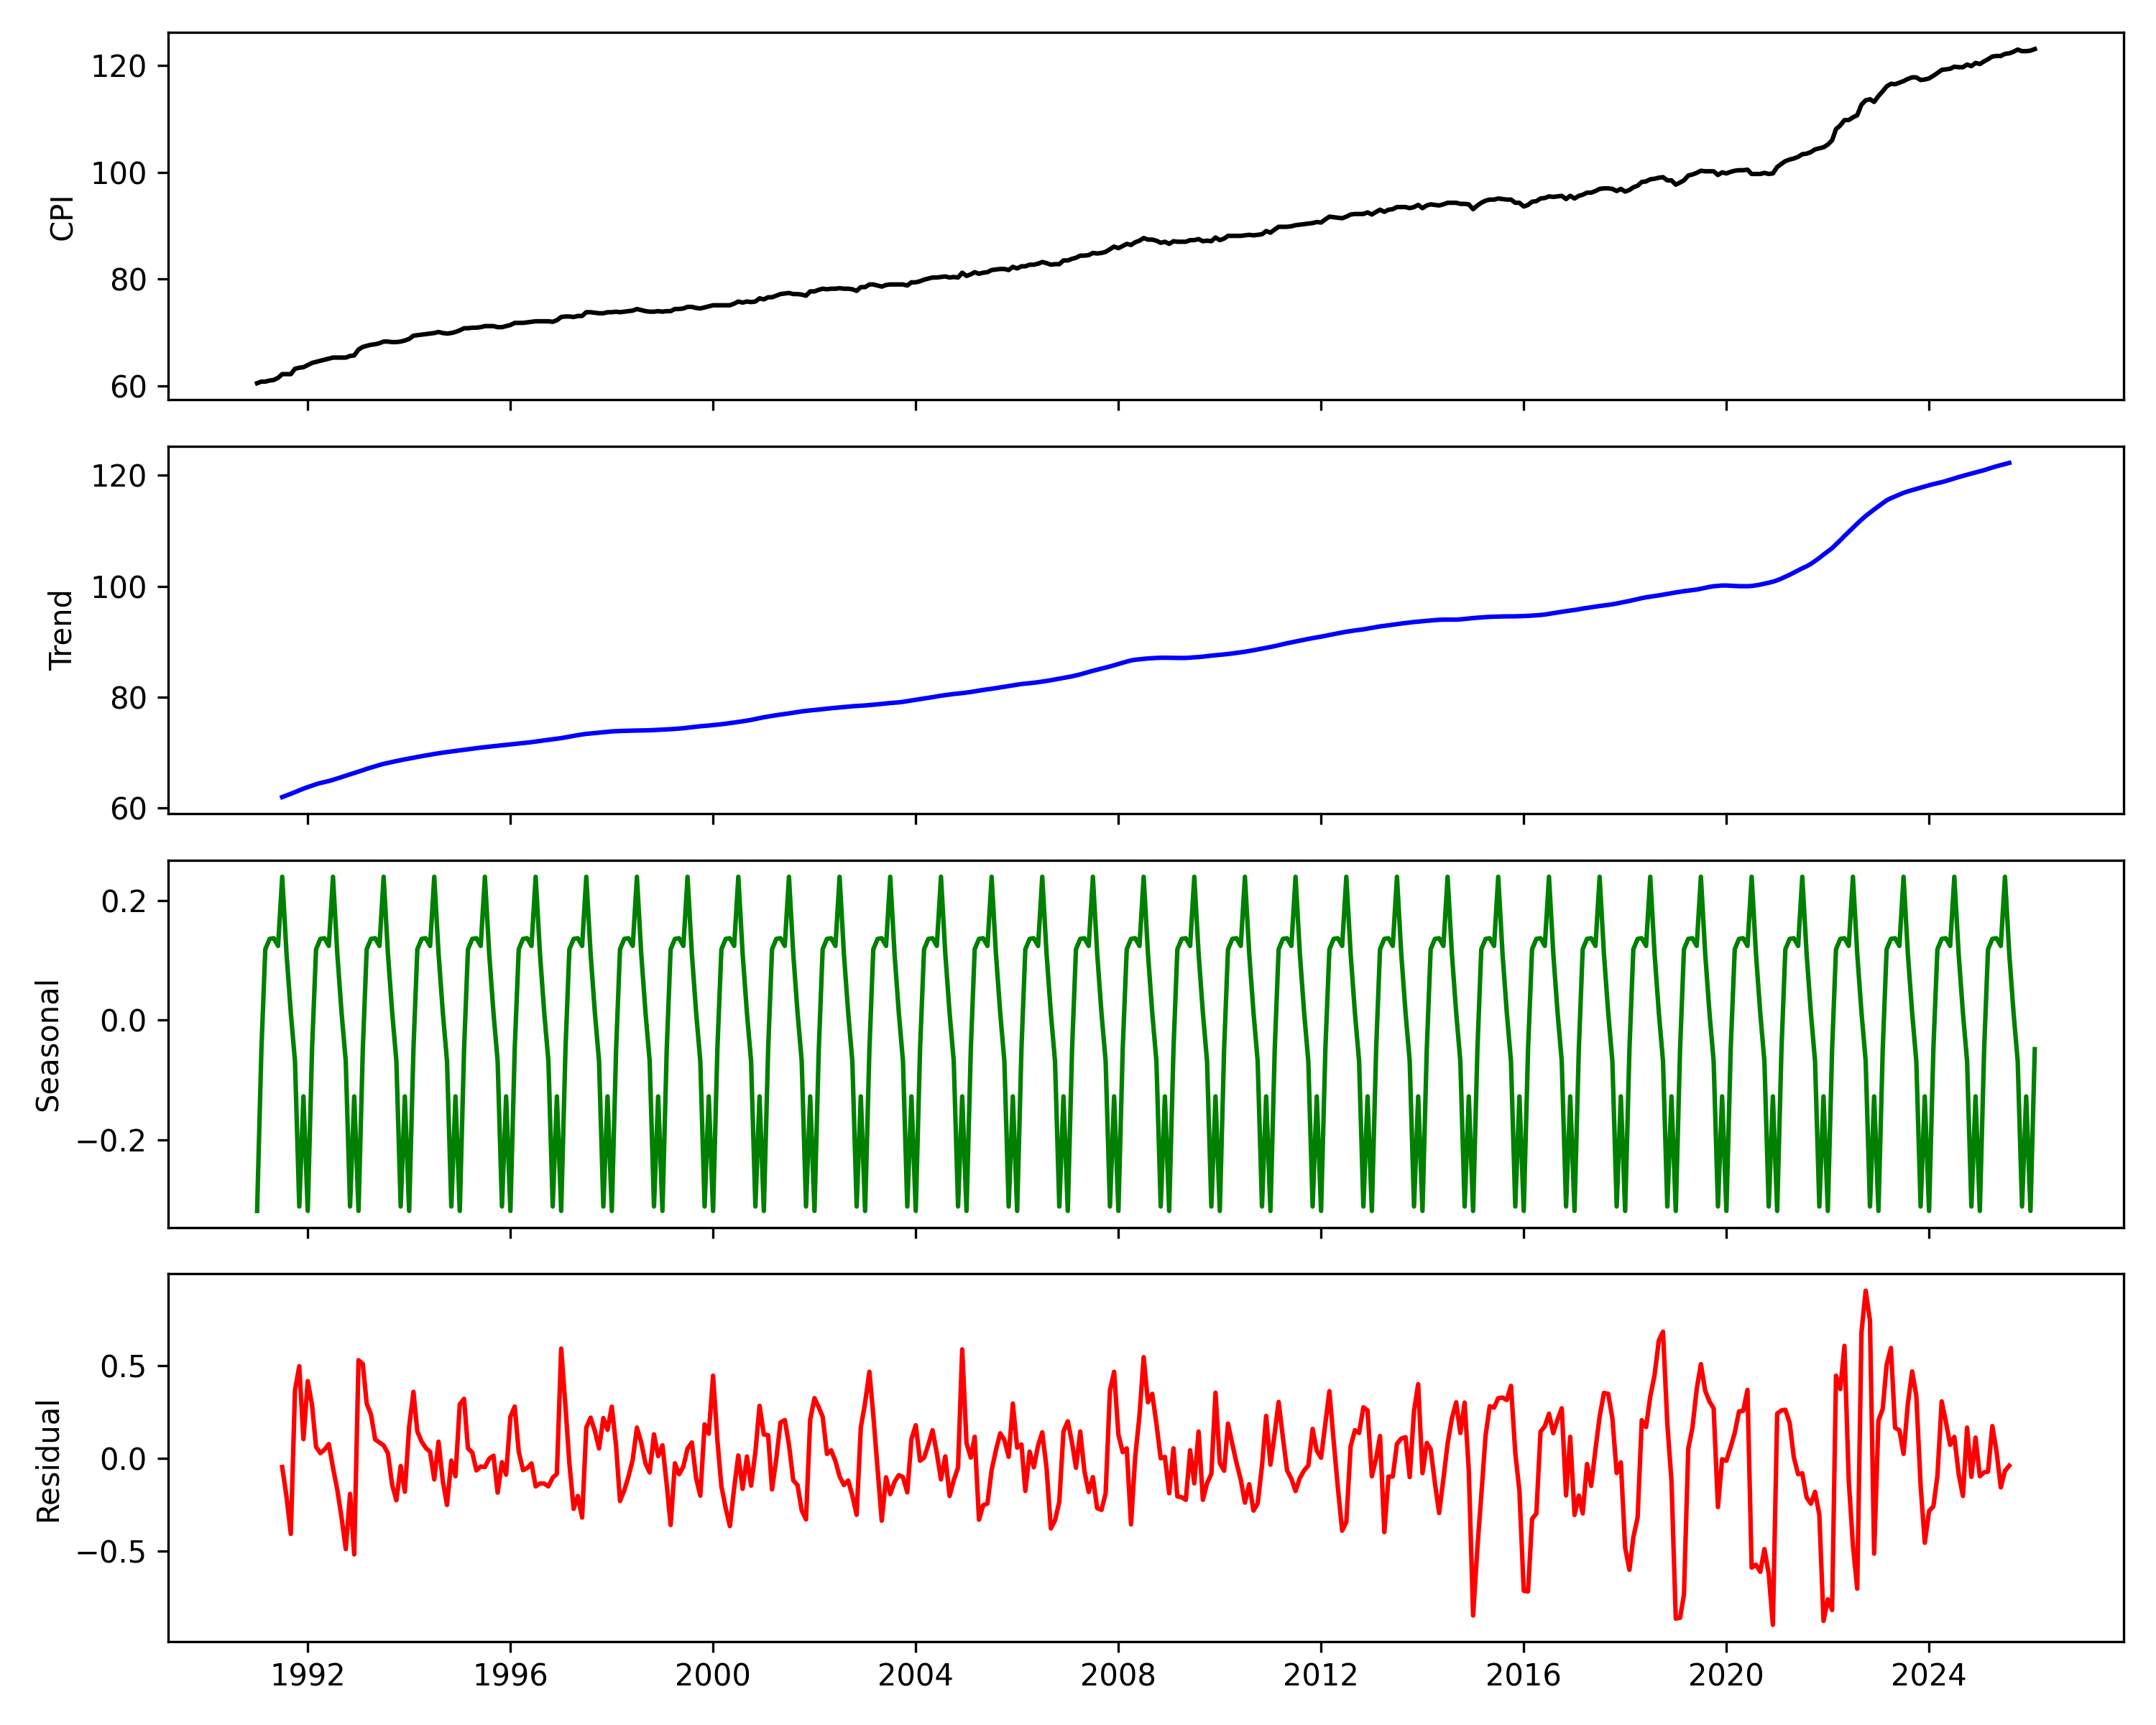
\includegraphics[width=0.9\textwidth]{../../Images/decomposition.png}
    \caption{Time Series Decomposition of the CPI dataset, illustrating the fundamental components modeled by the ETS framework: the observed CPI, the underlying Trend, the cyclic Seasonality, and the stochastic Residual Error. Source: own visualization based on Destatis GENESIS table 61111-0002 \cite{DestatisCPIQuality2023,DestatisCPIWeighting2023}.}
    \label{fig:ets_decomposition}
\end{figure}

The state transition mechanics are mapped in Figure~\ref{fig:ets_tikz}. Instead of relying on raw lags, the previous observation $y_{t-1}$ updates the distinct internal states governed by three crucial smoothing parameters: $\alpha$ dictates how heavily the new data shifts the baseline Level, $\beta$ dictates how much the long-term Trend slope adjusts, and $\gamma$ dictates the magnitude of the update to the periodic Seasonal cycle.

\begin{figure}[htbp]
\centering
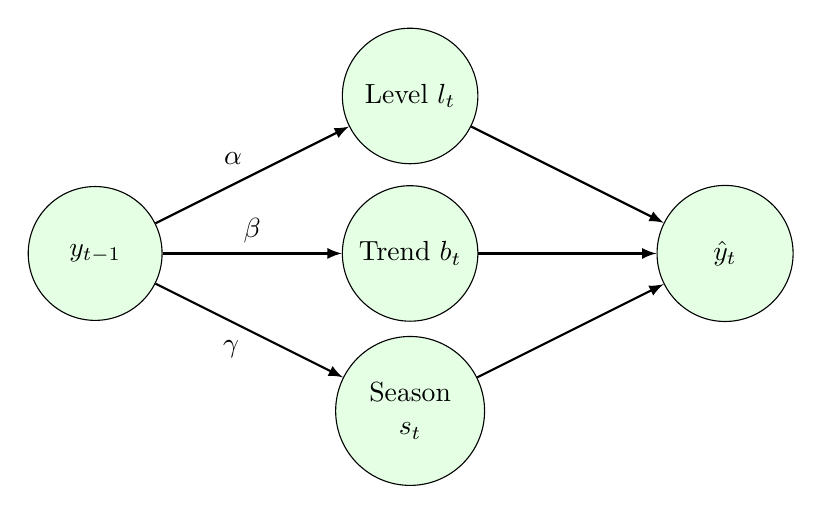
\begin{tikzpicture}[
    state/.style={circle, draw, fill=green!10, text width=4em, text centered, minimum height=4em},
    line/.style={draw, -latex, thick}
]
    \node [state] (y_t) at (0,0) {$y_{t-1}$};
    
    \node [state] (level) at (4,2) {Level $l_t$};
    \node [state] (trend) at (4,0) {Trend $b_t$};
    \node [state] (season) at (4,-2) {Season $s_t$};
    
    \node [state] (y_next) at (8,0) {$\hat{y}_{t}$};
    
    \draw [line] (y_t) -- (level) node[midway, above left] {$\alpha$};
    \draw [line] (y_t) -- (trend) node[midway, above] {$\beta$};
    \draw [line] (y_t) -- (season) node[midway, below left] {$\gamma$};
    
    \draw [line] (level) -- (y_next);
    \draw [line] (trend) -- (y_next);
    \draw [line] (season) -- (y_next);
\end{tikzpicture}

\caption{State transition diagram for ETS. Past observations update the distinct internal states governed by mathematical smoothing parameters ($\alpha, \beta, \gamma$), which are then recombined to produce the forecast $\hat{y}_t$. Source: own diagram based on exponential smoothing state-space formulations \cite{Hyndman2021}.}
\label{fig:ets_tikz}
\end{figure}

\section{Applications}
Exponential smoothing is arguably the most widely applied forecasting technique in industry today, particularly in automated forecasting environments, supply chain management, inventory control, and retail demand forecasting. The method gained prominent popularity because it requires minimal tuning compared to ARIMA models, naturally handles data with slowly evolving or non-stationary trends, and operates computationally faster on large arrays of parallel time series. The \texttt{forecast::ets} function developed by Rob Hyndman in R codified its dominance in the data science landscape.

\section{Relevance}
In this study modeling the Consumer Price Index (CPI) of Germany, the ETS framework proved to be the most accurate methodology, achieving a test Root Mean Squared Error (RMSE) of $0.7697$, decisively outperforming both the standard ARIMA ($1.3262$) and the seasonal SARIMA ($1.1909$). This success can be directly attributed to the structural properties of macroeconomic inflationary data. While inflation trends do shift, they tend to evolve smoothly rather than abruptly. The exponential smoothing mechanism inherent to ETS adapts gracefully to these gradual, non-linear level and trend shifts without requiring the explicit differencing steps mandated by ARIMA (which can over-difference and destroy valid historical signal). Moreover, ETS multiplicative configurations can natively model proportional changes in variance over long time horizons, a common macroeconomic trait where higher index values inherently correspond to larger absolute fluctuations.

\section{Hyperparameters}
The ETS framework discards discrete lag orders $(p,d,q)$ in favor of modeling the mathematical interactions between three core structural elements. Each element is categorized by its form:
\begin{itemize}
    \item \textbf{Error (E):} Determines how the residual stochastic noise affects the state equations. It can be Additive (A) or Multiplicative (M).
    \item \textbf{Trend (T):} Models the long-term progression of the series. It can be None (N), Additive (A), Multiplicative (M), or Damped (Ad/Md), allowing the trend to flatten out over a specific horizon.
    \item \textbf{Seasonality (S):} Accounts for periodic fluctuations overlaying the trend. It can be None (N), Additive (A), or Multiplicative (M).
    \item \textbf{Smoothing Parameters ($\alpha, \beta, \gamma$):} Internal coefficients bound between $0$ and $1$ determining how quickly the level, trend, and seasonal components update based on the newest observation. A value near $1$ assigns massive weight to the most recent error (rapid adaptation), while a value near $0$ relies heavily on historical inertia (smooth persistence). These are typically estimated automatically via maximum likelihood estimation (MLE).
\end{itemize}

\section{Requirements}
ETS is a highly versatile methodology. A primary advantage over ARIMA is that the data does not strictly need to be rendered stationary prior to modeling, as ETS inherently models and incorporates the non-stationary trend and seasonal components within its state equations. However, structural constraints do exist. For any model configuration containing a Multiplicative Error, Trend, or Seasonal term, the entire time series array must be strictly positive (i.e., $y_t > 0 \ \forall \ t$), as the framework divides states by previous states to calculate proportional impacts. Moreover, a robust seasonal frequency metadata parameter is required if the Seasonality component is active.

\section{Input}
The input consists of a univariate sequence, optimally structured as a \texttt{pandas.Series} with a continuous chronological index. For seasonal modeling variants, the frequency (e.g., $s=12$ for monthly cycles) must be mathematically declared prior to model estimation.

\section{Output}
The primary output is a statistically generated forecast trajectory. Because modern ETS models the entire data-generating process via defined state-space equations (rather than heuristic smoothing), it also robustly generates prediction intervals based on the estimated variance of the selected Error type, providing both point forecasts and confidence bounds. It also yields the extracted internal states (Level, Trend, Seasonality), offering a high degree of explainability to stakeholders analyzing how the forecast was derived.

\section{Example with a program}
The following snippet demonstrates fitting a fully Additive ETS model using the \texttt{statsmodels} framework:

\begin{Python}[caption={ETS Implementation using Statsmodels}, label={lst:ets_python}]
import pandas as pd
from statsmodels.tsa.exponential_smoothing.ets import ETSModel

# 'cpi_series' is a pandas Series indexed by a monthly DatetimeIndex
# Time series must contain no missing values for proper state initialization.
cpi_series = pd.Series([105.1, 105.4, 105.8, 106.2, 106.5])

# Initialize an ETS(A,A,A) model (Holt-Winters Additive):
# Error=Additive, Trend=Additive, Seasonality=Additive
model = ETSModel(endog=cpi_series, 
                 error="add", 
                 trend="add", 
                 seasonal="add", 
                 damped_trend=False,
                 seasonal_periods=12)

# Fit the model using maximum likelihood to optimize alpha, beta, gamma
fitted_model = model.fit(disp=False)

# Forecast the next 12 periods and retrieve the prediction result object
forecast_result = fitted_model.get_prediction(start=len(cpi_series), end=len(cpi_series)+11)
predictions = forecast_result.predicted_mean
conf_ints = forecast_result.pred_int(alpha=0.05) # 95% CI

print(predictions)
\end{Python}

\section{Further Reading}
\begin{itemize}
    \item Hyndman, R. J., Koehler, A. B., Ord, J. K., \& Snyder, R. D. (2008). \textit{Forecasting with Exponential Smoothing: The State Space Approach}. Springer. (The definitive textbook mapping simple smoothing to the rigorous ETS state-space framework). \cite{Hyndman2018}
    \item Hyndman, R. J., \& Athanasopoulos, G. (2018). \textit{Forecasting: Principles and Practice} (2nd ed.). OTexts. Available at \url{https://otexts.com/fpp2/ets.html}.
\end{itemize}
